
\documentclass[25pt, a0paper, portrait]{tikzposter} %Options for format can be included here

\tikzposterlatexaffectionproofoff

\usepackage[none]{hyphenat} %stop hyphenation

 % Title, Author, Institute
\title{How does grid-resolution modulate geomorphic processes?}
\author{Stuart W. D. Grieve \large{\texttt{(s.grieve@ed.ac.uk)}}, \LARGE Simon M. Mudd, David T. Milodowski, Fiona J. Clubb \& David J. Furbish}
\institute{Univerity of Edinburgh, Vanderbilt University}
\titlegraphic{
  \raisebox{-0.5\height}{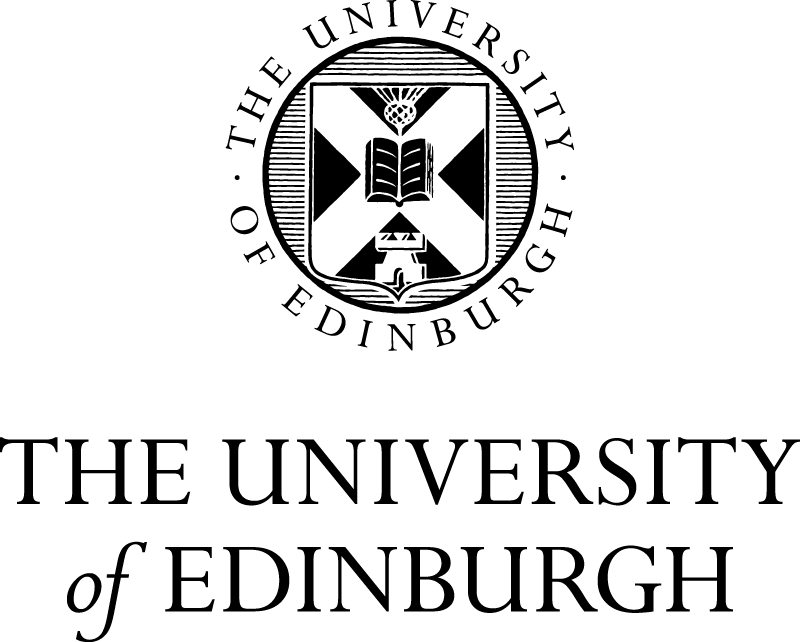
\includegraphics[height=4.0cm]{./logos/UoE_Centre_Logo.png}}
  \hfill
  \raisebox{-0.5\height}{
\includegraphics[height=4.0cm]{./logos/vanderbilt2.jpg}}
  \hfill
  \raisebox{-0.5\height}{
\includegraphics[height=3.0cm]{./logos/nerc-logo.eps}}
  \hfill
  \raisebox{-0.5\height}{
\includegraphics[height=2.6cm]{./logos/ARL_logo.png}}
  \hfill
  \raisebox{-0.5\height}{
\includegraphics[height=3.4cm]{./logos/Carn.pdf}}
  \hfill
  \raisebox{-0.5\height}{
\includegraphics[height=3.6cm]{./logos/nsf1.eps}}
  \hfill
  \raisebox{-0.5\height}{
\includegraphics[height=3.0cm]{./logos/LSD-logo_horizontal.png}}
  \hfill
}


\settitle{ \centering \vbox{
\color{titlefgcolor} {\bfseries \Huge \sc \@title \par}
\vspace*{1em}
{\LARGE \@author \par} \vspace*{1.5em} \@titlegraphic \\[\TP@titlegraphictotitledistance]
}}

 %Choose Layout
\usetheme{Rays}

\begin{document}

 % Title block with title, author, logo, etc.
\maketitle[width=800mm]


\begin{columns}

 % FIRST column
\column{0.5}% Width set relative to text width

\block[titleleft]{Motivation}{
\LARGE
Digital elevation models (DEMs) are an integral part of modern geomorphic research yet in many locations high resolution data are not available.

\begin{tikzfigure}
  \label{hillshade_fig}
  \includegraphics[width=38cm]{./figures/HS_fig.png}
\end{tikzfigure}
\textbf{Is it possible to perform geomorphic analysis on low resolution data?}
}

\block[titleleft]{Channel extraction}{
Channels can be extracted from high resolution DEMs using methods based on the \textbf{curvature of hillslopes} or the \textbf{topographic signature of fluvial processes}. Our ability to apply these methods to low resolution data can be quantified using indices of quality, which measure rates of over- and under-prediction of network extent.
\vspace*{-0.5em}
\begin{tikzfigure}
  \label{chan_fig}
  \includegraphics[width=38cm]{./figures/Chan_poster.png}
\end{tikzfigure}
\LARGE
\textbf{Drainage density is reduced as resolution decreases, but the geometric method preserves more of the channel network.}

}

\block[titleleft]{Sediment transport coefficient}{
The sediment transport coefficient ($D$) can be calculated for a hillslope, given an independent constraint on the erosion rate, using measurements of \textbf{hilltop curvature.}

\begin{tikzfigure}
  \label{diff_fig}
  \includegraphics[width=36cm]{./figures/finaldiff.png}
\end{tikzfigure}

\LARGE
\textbf{Measurements of $D$ from topographic data depend on ridgeline width in addition to data resolution.}

}

 % SECOND column
\column{0.5}

\block[titleright]{Curvature}{
Landscape curvature is a common measurement performed on topographic data, used to identify \textbf{channel networks}, estimate \textbf{erosion rates} and \textbf{sediment transport coefficients.}

\begin{tikzfigure}
  \label{spatial_curv_fig}
  \includegraphics[width=30cm]{./figures/curvature.png}
\end{tikzfigure}

\begin{tikzfigure}
  \label{curv_fig}
  \includegraphics[width=30cm]{./figures/curv_fig.png}
\end{tikzfigure}
\LARGE
\textbf{As grid-resolution is decreased, extreme curvatures are lost, yet the majority of the curvature distribution is unchanged.}

}

\block[titleright]{Hillslope length and relief}{
Measuring hillslope length and relief yields important insights into \textbf{sediment transport}, \textbf{landscape evolution} and \textbf{landslide hazard.} These metrics are tested using channel networks extracted from 1 metre and reduced resolution topographic data.

\begin{tikzfigure}
  \label{lh_fig}
  \includegraphics[width=38cm]{./figures/sc_lh.png}
\end{tikzfigure}
\LARGE
\textbf{The measurement of hillslope length and relief is stable up to resolutions in excess of 10 metres.}
}

\block[titleright]{More information}{

\textbf{Read the paper:} How does grid-resolution modulate the topographic expression of geomorphic processes?, Earth Surf. Dynam., 4, \textit{627-653}, 2016.\\\\
\textbf{Get the software:} LSDTopoTools.github.io
\vspace*{0.55em}
}

\end{columns}

\end{document}

\endinput
